%%========================Introducao================================%%
\section{Dobramento de Proteínas}

%%========================Objetivo================================%%
\subsection{Proteínas}
\frame{
	\frametitle{Proteínas}

		\begin{itemize}
			\item 	Estruturas compostas por uma ou mais cadeias de aminoácidos.
			\item 	Exercem um papel fundamental na natureza.
			\item   Responsáveis por muitas funções importantes da células vivas.
			\item 	São produtos de um processo chamado dobramento de proteínas.
			\item	Inicia a partir de uma cadeia de aminoácidos inicialmente desdobrada que será transformada em sua estrutura final/nativa.
		\end{itemize}

}

\subsection{Problema de Dobramento Proteínas}
\frame{
	\frametitle{Problema de Dobramento de Proteínas}
		\begin{itemize}
			\item Preocupa-se em entender o processo de dobramento das proteínas.
			\item Também trata da predição das estruturas de proteínas.
			\item A predição das estruturas tem um amplo campo de aplicações:
			\begin{itemize}
				\item Síntese de novas proteínas e dobramentos.
				\item Síntese de novas drogas baseada nas estruturas.
				\item Obtenção de estruturas a partir de dados
				incompletos de ressonância magnética nuclear.
			\end{itemize}
			\item A determinação da estrutura nativa de proteínas é uma tarefa desafiadora até mesmo para modernos super computadores.
			\item Trata-se de um problema $NP$-Completo.
		\end{itemize}
}

\frame{
	\frametitle{Modelos de Representação de Proteínas}
		\begin{itemize}
			\item Diferentes modelos para representar proteínas existem.
			\item Modelos extremamente detalhados são computacionalmente caros.
			\item Modelos simplificados são largamente utilizados por pesquisadores por conta de sua simplicidade em representar as proteínas.
			\item Modelo Hidrofóbico-Polar (HP).
		\end{itemize}

}


\begin{frame}[allowframebreaks]{Modelo Hidrofóbico-Polar}
	

		\begin{itemize}
			\item Generaliza os aminoácidos que compõem as proteínas em apenas dois aminoácidos: hidrofóbicos H ou polares P.
			\item Utiliza um \textit{grid} 2d ou um cubo 3d para representar as possíveis conformações de uma proteína.
			\item No modelo HP existem 3 interações entre os aminoácidos H-P, P-P e H-H.
			\item Para calcular a energia de uma conformação no modelo HP é necessário avaliar a quantidade de interações hidrofóbicas (H-H) entre aminoácidos não consecutivos na sequência.
		\end{itemize}
		
		\begin{figure}[!htb]
			\centering
			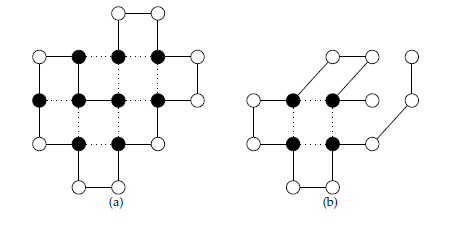
\includegraphics[scale=.8]{figuras/modeloHPExemplo.png}
			\caption{Exemplos de representação de proteínas utilizando os modelos HP 2D-HP (a) e 3D-HP (b). Fonte: Adaptado de \cite{santanna2008} }
			\label{fig:exemploModeloHP}
		\end{figure}

\end{frame}



\begin{frame}[allowframebreaks]{Representação do Problema}
	
	\begin{itemize}
		\item Existem várias maneiras de representar as conformações no modelo HP.
		\item 	Coordenadas relativas: O conjunto de movimentos possíveis para a grade 2D é definido por $\{F,E,D\}$, que correspondem aos movimentos: frente (continuar no mesmo sentido do aminoácido anterior), à esquerda e à direita. 
		\item Geralmente se utiliza uma codificação utilizando números inteiros, como por exemplo:  F$->$0, E$->$1 e D$->$2. 
	\end{itemize}
	
	\begin{figure}[!htb]
		\centering
		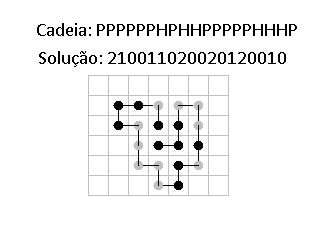
\includegraphics[scale=.8]{figuras/ExemploCodificacao.png}
		\caption{Exemplo de conformação gerada por uma solução codificada utilizando coordenadas relativas para uma cadeia de 20 aminoácidos.  Fonte: Autoria Própria }
		\label{fig:exemploCodificacao}
	\end{figure}



	
\end{frame}

	
